%%%%%%%%%%%%%%%%%%%%%%%%%%%%%%%%%%%%%%%%%
% Beamer Presentation
% LaTeX Template
% Version 1.0 (10/11/12)
%
% This template has been downloaded from:
% http://www.LaTeXTemplates.com
%
% License:
% CC BY-NC-SA 3.0 (http://creativecommons.org/licenses/by-nc-sa/3.0/)
%
%%%%%%%%%%%%%%%%%%%%%%%%%%%%%%%%%%%%%%%%%

%----------------------------------------------------------------------------------------
%	PACKAGES AND THEMES
%----------------------------------------------------------------------------------------

\documentclass{beamer}

\mode<presentation> {

% The Beamer class comes with a number of default slide themes
% which change the colors and layouts of slides. Below this is a list
% of all the themes, uncomment each in turn to see what they look like.

%\usetheme{default}
%\usetheme{AnnArbor}
%\usetheme{Antibes}
%\usetheme{Bergen}
%\usetheme{Berkeley}
%\usetheme{Berlin}
%\usetheme{Boadilla}
%\usetheme{CambridgeUS}
%\usetheme{Copenhagen}
%\usetheme{Darmstadt}
%\usetheme{Dresden}
%\usetheme{Frankfurt}
%\usetheme{Goettingen}
%\usetheme{Hannover}
\usetheme{Ilmenau}
%\usetheme{JuanLesPins}
%\usetheme{Luebeck}
%\usetheme{Madrid}
%\usetheme{Malmoe}
%\usetheme{Marburg}
%\usetheme{Montpellier}
%\usetheme{PaloAlto}
%\usetheme{Pittsburgh}
%\usetheme{Rochester}
%\usetheme{Singapore}
%\usetheme{Szeged}
%\usetheme{Warsaw}

% As well as themes, the Beamer class has a number of color themes
% for any slide theme. Uncomment each of these in turn to see how it
% changes the colors of your current slide theme.

%\usecolortheme{albatross}
%\usecolortheme{beaver}
%\usecolortheme{beetle}
%\usecolortheme{crane}
%\usecolortheme{dolphin}
%\usecolortheme{dove}
%\usecolortheme{fly}
%\usecolortheme{lily}
%\usecolortheme{orchid}
%\usecolortheme{rose}
%\usecolortheme{seagull}
%\usecolortheme{seahorse}
%\usecolortheme{whale}
%\usecolortheme{wolverine}

%\setbeamertemplate{footline} % To remove the footer line in all slides uncomment this line
\setbeamertemplate{footline}[page number] % To replace the footer line in all slides with a simple slide count uncomment this line

\setbeamertemplate{navigation symbols}{} % To remove the navigation symbols from the bottom of all slides uncomment this line
}

\usepackage{graphicx} % Allows including images
\usepackage{booktabs} % Allows the use of \toprule, \midrule and \bottomrule in tables
%\usepackage {tikz}
\usepackage{tkz-graph}
\GraphInit[vstyle = Shade]
\tikzset{
  LabelStyle/.style = { rectangle, rounded corners, draw,
                        minimum width = 2em, fill = yellow!50,
                        text = red, font = \bfseries },
  VertexStyle/.append style = { inner sep=5pt,
                                font = \normalsize\bfseries},
  EdgeStyle/.append style = {->, bend left} }
\usetikzlibrary {positioning}
%\usepackage {xcolor}
\definecolor {processblue}{cmyk}{0.96,0,0,0}
%----------------------------------------------------------------------------------------
%	TITLE PAGE
%----------------------------------------------------------------------------------------

\title[Short title]{Superbubbles, Ultrabubbles and Cacti by Paten, Novak, et al.} % The short title appears at the bottom of every slide, the full title is only on the title page

\author{Nathanael Roy} % Your name
\institute[UC Riverside] % Your institution as it will appear on the bottom of every slide, may be shorthand to save space
{
University of California \\ % Your institution for the title page
\medskip
}
\date{\today} % Date, can be changed to a custom date

\begin{document}

\begin{frame}
\titlepage % Print the title page as the first slide
\end{frame}

\begin{frame}
\frametitle{Overview} % Table of contents slide, comment this block out to remove it
\tableofcontents % Throughout your presentation, if you choose to use \section{} and \subsection{} commands, these will automatically be printed on this slide as an overview of your presentation
\end{frame}

%----------------------------------------------------------------------------------------
%	PRESENTATION SLIDES
%----------------------------------------------------------------------------------------

%------------------------------------------------

\section{Nucleotide Sequences as Graphs}
\begin{frame}{Introduction}
    \begin{itemize}
        \item Graphs: Possible Sequencing of Nucleotides
        \item Example: Hidden Markov Model
        \item Previous work: Bubble
    \end{itemize}
    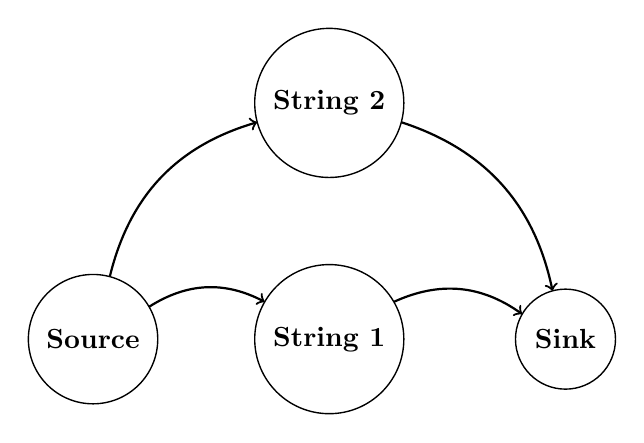
\begin{tikzpicture}
  \SetGraphUnit{3}
  \Vertex{String 1}
  \WE(String 1){Source}
  \EA(String 1){Sink}
  \NO(String 1){String 2}
  \Edge (Source)(String 1)
  \Edge (Source)(String 2)
  \Edge (String 1)(Sink)
  \Edge (String 2)(Sink)
\end{tikzpicture}
\end{frame}
\section{Directed, Bidirected, and Biedged Graphs}
\begin{frame}{Bidirected, Digraph, and Biedged Graph}
\begin{itemize}
    \item  Bidirected Graph $D= (V_D,E_D)$: each endpoint of every edge has an independent orientation indicating incidents with left or right side of a given vertex
    \item Digraph: Bidirectedgraph where each edge connects a left and right side
    \item Biedged Graph: A graph with two types of edges, black and gray, such that each vertex is incident with at most one black edge
    \begin{block}{Lemma 1}
    For any acyclic biedged graph B(D) there exists an isomorphic biedged graph B(D) such that D is a directed acyclic graph
    \end{block}
\end{itemize}
\end{frame}
\begin{frame}{Graph Examples}
\begin{figure}[H]
\centering
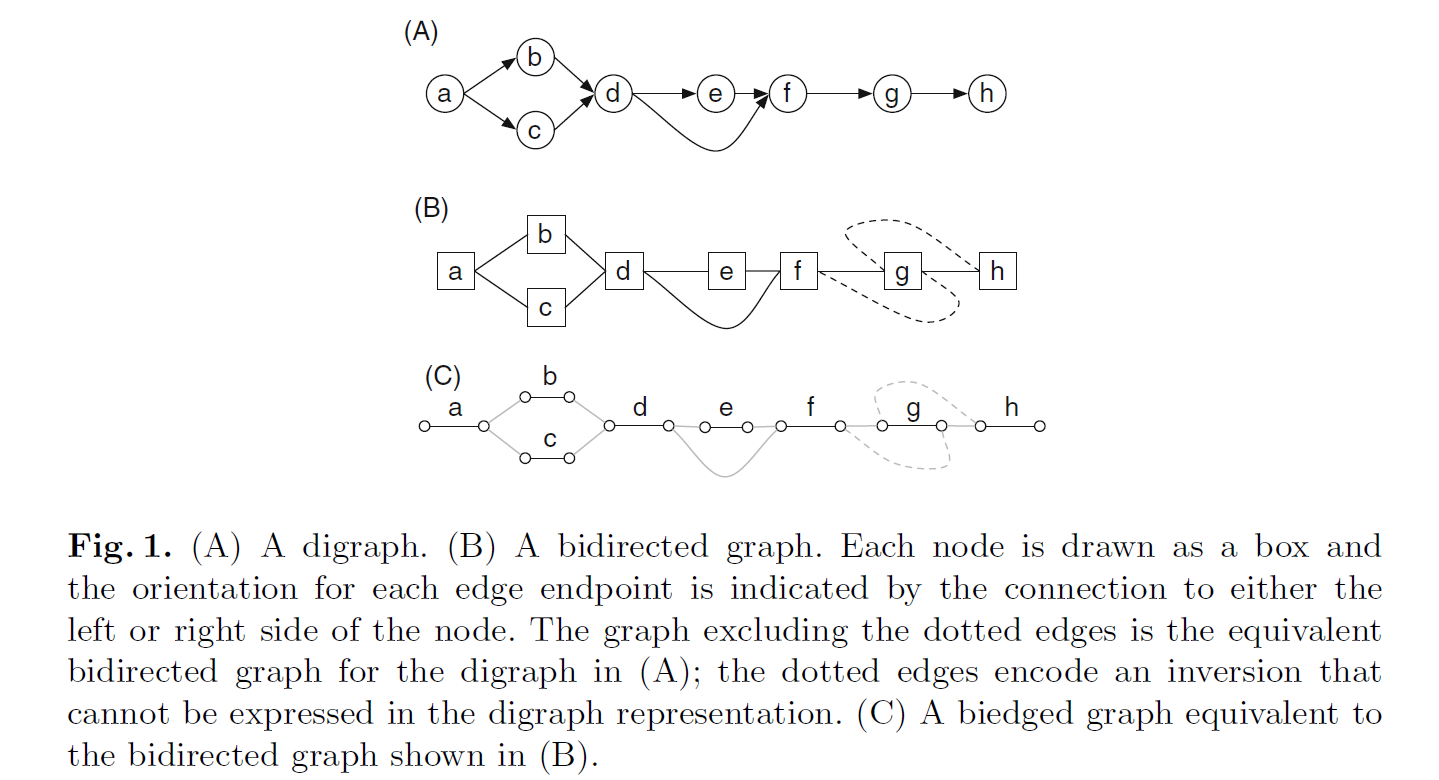
\includegraphics[width=110mm]{DiBidiBiedge.png}
\end{figure}
\end{frame}
\section{Superbubbles, Snarls and Ultrabubbles}
\begin{frame}{Superbubble}
    A Superbubble is a more complex subgraph type in which a set of paths start and end at common sink nodes:
\begin{tikzpicture}
  \SetGraphUnit{3}
  \Vertex{X}
  \WE(String 1){Source}
  \EA(String 1){Sink}
  \Edge (Source)(X)
  \Edge (X)(Sink)
\end{tikzpicture}
\begin{itemize}
    \item reachability
    \item matching
    \item acyclicity 
    \item minimality
\end{itemize}
\end{frame}
\begin{frame}{Superbubble Example}
\begin{figure}[H]
\centering
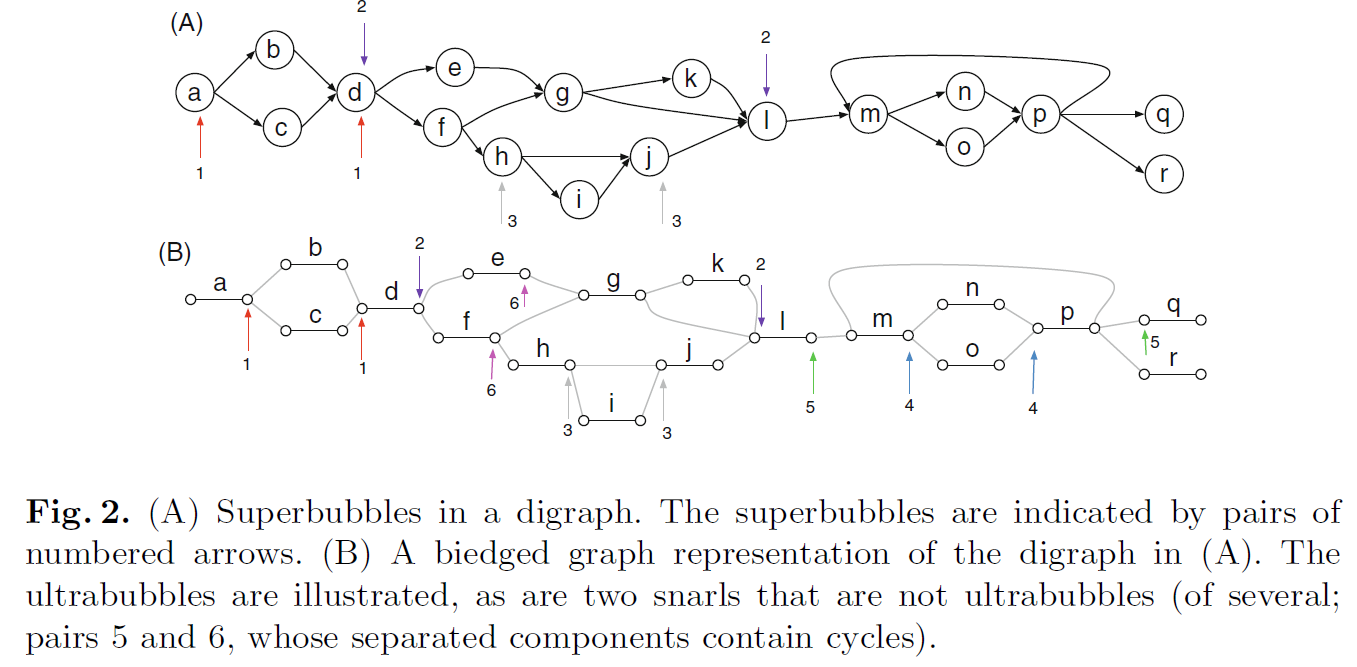
\includegraphics[width=110mm]{Superbubbles.png}
\end{figure}

\end{frame}
\begin{frame}{Snarl}
In order to generalize a superbubble
\begin{itemize}
    \item Snarl: 2 Black-Edge-Connected graph (2-BEC)
    \item Two non-opposite vertices are a snarl if
    \begin{itemize}
        \item separable
        \item minimality
    \end{itemize}
    \item Tip: A vertex on a biedged graph with a grey edge
    \item Ultrabubble: If the subgraph X induced by a snarl is acyclic and contains no tips
    \begin{block}{Lemma 2}
    For any superbubble (x,y) in a digraph D, the pair set {x' = (x,right),y'=(y,left)} is an ultrabubble in B(D), a biedged graph
    \end{block}
\end{itemize}
\end{frame}
\section{Cactus Graphs}
\begin{frame}{Cactus Graph}
    \begin{itemize}
        \item Definition: A graph in which any two vertices are at most two-edge connected
        \item Each edge is apart of at most one simple cycle
        \item Suppose we have a graph G which is not a cactus graph. 
        \item We can create a mapping from $G \rightarrow G'$; a graph homomorphism that maps each vertex in set $V_G$ into $V_G'$
        \item The set of vertices mapped to in $G'$ is 2 edge connected 
    \end{itemize}
\end{frame}

\begin{frame}{Chain Pairs, Bridge Pairs, and Bridge Forest}
    \begin{itemize}
        \item Chain pair
        \begin{itemize}
            \item Project to same vertex in cactus homomorphism
            \item black edges project to same simple cycle
        \end{itemize}
        \item Bridge Forest
        \begin{itemize}
            \item Graph resulting from contracting simple cycles
        \end{itemize}
        \item Bridge pair
        \begin{itemize}
            \item If pair of vertices project to the same vertex in bridge forest  and both incident black edges are bridges
        \end{itemize}
    \end{itemize}
    
\end{frame}
\begin{frame}{Biedged graph, Contracted Gray Edges, Cactus Graph, Bridge Forest}
\begin{figure}[H]
\centering
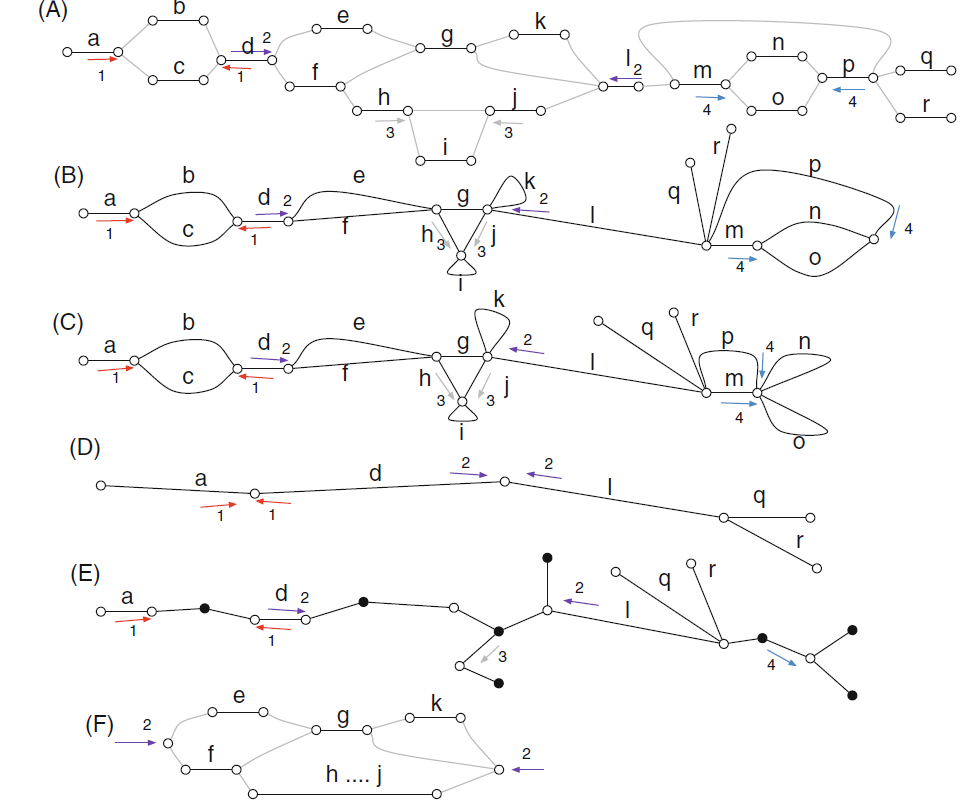
\includegraphics[width=85mm]{CactusBridgeForest.png}
\end{figure}
\end{frame}
\section{Lemmas and Theorems for Algorithm}
\begin{frame}{Useful Theorems and Lemmas}
\begin{block}{Theorem}
The set of snarls in B(D) a bidirected graph is equal to the union of chain pairs and bridge pairs
\end{block}
\begin{block}{Lemma}
A snarl {x,y} in a bidirected graph is an ultrabubble iff its net graph and the net graph of each snarl contained in {x,y} is acyclic and bridgeless
\end{block}

\begin{block}{Lemma}
For a chain pair or bridge pair {x,y} in B(D) the set of contained snarls is equal to its contained chain pairs
\end{block}
\begin{block}{Theorem}
A snarl {x,y} in B(D) a bidirected graph is an ultrabubble iff its net graph and the net graph of each its contained chain pairs is acyclic and brdgeless (follows immediately from two lemmas)
\end{block}
\end{frame}
\begin{frame}{Algorithm}
Given a bidirected graph $B(D)$ we can
\begin{enumerate}
    \item Calculate the Cactus Graph $C(D)$
    \item Calculate the Cactus Tree
    \item Use depth first search to determine, for each chain pair whether its net graph and the net graph contained is acyclic and bridgeless (using Theorem to determine ultrabubble) 
    \item Calculate Bridge Forest
    \item For each vertex x in bridge forest, calculate if net graph and contained chain pairs are acyclic and bridgeless reporting bridge pair as ultrabubble if true.
\end{enumerate}
\end{frame}

\section{Implementation}
 \begin{frame}{Time Complexity and Implementation for Genetic Sites}
     The time complexity for this problem is O(\#edges + \#vertices) in a bidirected graph. 
     
     Superbubbles have a nested relationship: Easy to get a tree type structure given a graph
     
     Bidirected Graphs: Can be constructed from genome variation "sites" or alternatives at various parts of the genome. 
\end{frame}

\begin{frame}
\begin{figure}[H]
\centering
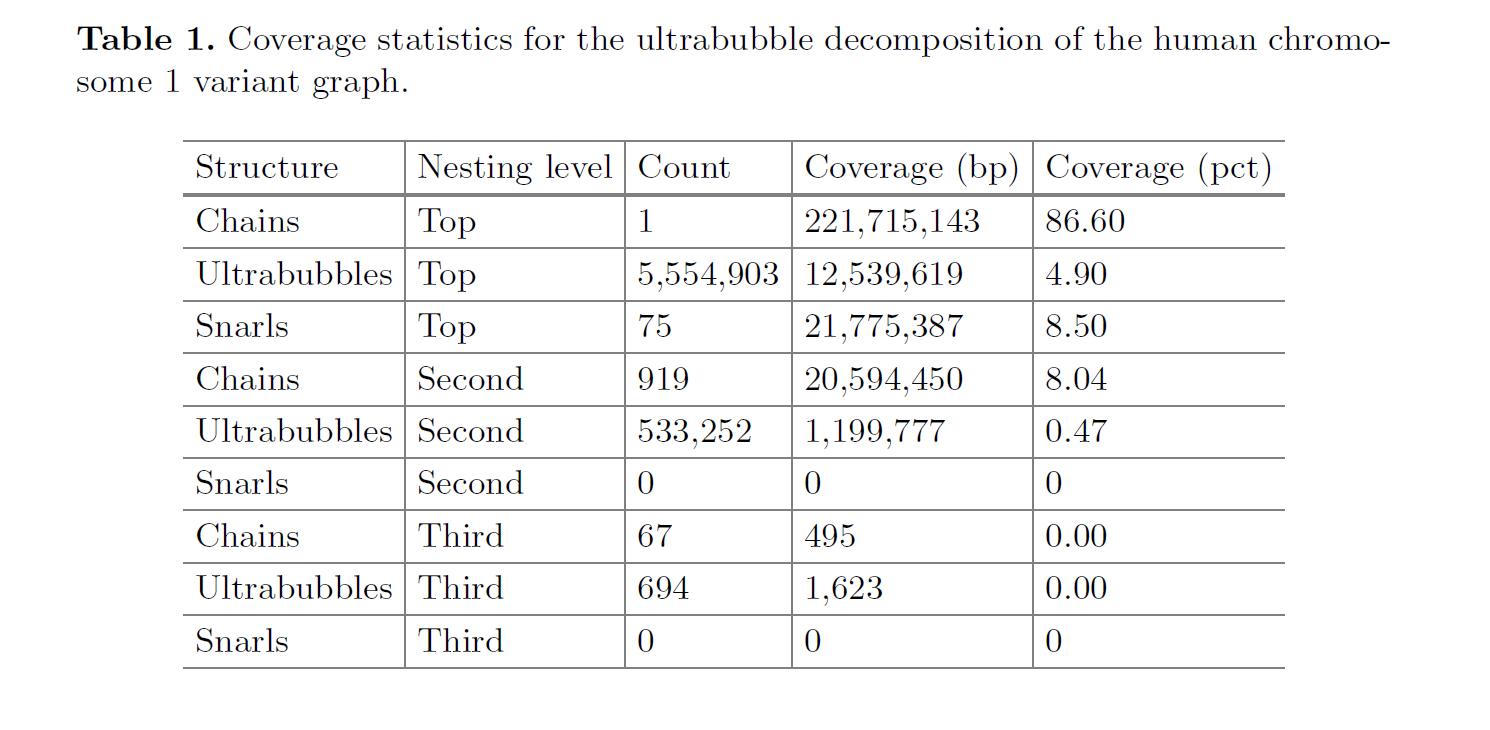
\includegraphics[width=110mm]{TableChr1.png}
\end{figure}
\end{frame}
\begin{frame}{Conclusions from Paper}
    \begin{itemize}
        \item Solves an important problem in using graphs to represent genetic variation
        \item Large majority of sites are either invariant or described by simple, top-level ultrabubbles
        \item More complex structures might be needed to represent inversions, translocations, etc.
        \item Other than subclassification, error correction algorithms can be used to reduce complexity of graph
    \end{itemize}
\end{frame}
\begin{frame}{My Takeaways}
    \begin{itemize}
        \item Top level ultrabubbles: only 4.9 percent, doesn't seem like majority
        \item Summary information to describe variation in genome 
        \item Interpretation of superbubbles, ultrabubbles, snarls, etc. unclear to me
        \item Outside resources needed to understand graph theory, simpler visualizations may have been nice
    \end{itemize}
\end{frame}

\begin{frame}{Useful Resources}
\begin{itemize}
    \item Paten, Benedict, et al. "Superbubbles, ultrabubbles, and cacti." Journal of Computational Biology 25.7 (2018): 649-663.
    \item sagemath.org or cocalc.com Software for using R and other programming languages to do graph theory
    \item https://www.youtube.com/user/DrSaradaHerke/

\end{itemize}
    
\end{frame}


\end{document}

\begin{frame}
\frametitle{Blocks of Highlighted Text}
\begin{block}{Block 1}
Lorem ipsum dolor sit amet, consectetur adipiscing elit. Integer lectus nisl, ultricies in feugiat rutrum, porttitor sit amet augue. Aliquam ut tortor mauris. Sed volutpat ante purus, quis accumsan dolor.
\end{block}

\begin{block}{Block 2}
Pellentesque sed tellus purus. Class aptent taciti sociosqu ad litora torquent per conubia nostra, per inceptos himenaeos. Vestibulum quis magna at risus dictum tempor eu vitae velit.
\end{block}

\begin{block}{Block 3}
Suspendisse tincidunt sagittis gravida. Curabitur condimentum, enim sed venenatis rutrum, ipsum neque consectetur orci, sed blandit justo nisi ac lacus.
\end{block}
\end{frame}

%------------------------------------------------

\begin{frame}
\frametitle{Multiple Columns}
\begin{columns}[c] % The "c" option specifies centered vertical alignment while the "t" option is used for top vertical alignment

\column{.45\textwidth} % Left column and width
\textbf{Heading}
\begin{enumerate}
\item Statement
\item Explanation
\item Example
\end{enumerate}

\column{.5\textwidth} % Right column and width
Lorem ipsum dolor sit amet, consectetur adipiscing elit. Integer lectus nisl, ultricies in feugiat rutrum, porttitor sit amet augue. Aliquam ut tortor mauris. Sed volutpat ante purus, quis accumsan dolor.

\end{columns}
\end{frame}

%------------------------------------------------
\section{Second Section}
%------------------------------------------------

\begin{frame}
\frametitle{Table}
\begin{table}
\begin{tabular}{l l l}
\toprule
\textbf{Treatments} & \textbf{Response 1} & \textbf{Response 2}\\
\midrule
Treatment 1 & 0.0003262 & 0.562 \\
Treatment 2 & 0.0015681 & 0.910 \\
Treatment 3 & 0.0009271 & 0.296 \\
\bottomrule
\end{tabular}
\caption{Table caption}
\end{table}
\end{frame}

%------------------------------------------------


\begin{frame}
\frametitle{References}
\footnotesize{
\begin{thebibliography}{99} % Beamer does not support BibTeX so references must be inserted manually as below
\bibitem[Smith, 2012]{p1} John Smith (2012)
\newblock Title of the publication
\newblock \emph{Journal Name} 12(3), 45 -- 678.
\end{thebibliography}
}
\end{frame}

%------------------------------------------------

\begin{frame}
\Huge{\centerline{The End}}
\end{frame}

%----------------------------------------------------------------------------------------
